\documentclass[11pt,twocolumn]{article}

\usepackage[hmargin=1.25cm, vmargin=1.5cm]{geometry} % Document margins

\usepackage{amsmath}
\usepackage{amsthm}
\usepackage{graphicx}
\usepackage{mathtools}
\usepackage{fullpage}
\usepackage{verbatim}

\title{Brownian Dynein Model}

\newcommand{\mn}{\scalebox{0.7}[1.0]{-}}

\begin{document}

\maketitle

\begin{figure}
  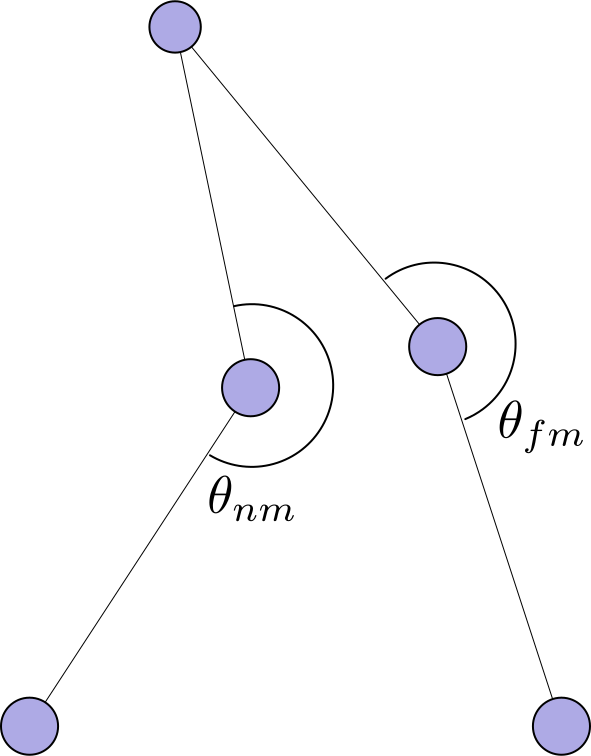
\includegraphics[width=\columnwidth]{../figures/code-bothbound}
  \caption{Angles used in both-bound case.}\label{fig:bothbound}
\end{figure}

In the both-bound case, we use two angles, as illustrated in
Fig.~\ref{fig:bothbound}.

\end{document}
